\section{Stack und Heap}

\subsection{»Dinge« und Stack}

\newcommand{\stackimgframe}[3]{
	\begin{frame}[t]{#1}
		\includegraphics[width=\linewidth]{images/#2}
		
		\begin{block}{}
			#3
		\end{block}
	\end{frame}
}

\begin{frame}[fragile]{Allokation auf Stack}
	\verb|TYPE name;| \hspace{1em} bzw. \hspace{1em} \verb|TYPE name(PARAMETER);|
	\begin{itemize}
		\item Alloziert das »Ding« vom Typ \verb|TYPE| auf dem Stack (den Speicher!).
		\item Ruft den Konstruktor von TYPE auf (und übergibt die PARAMETER).
		\item Führt den Namen \verb|name| für das »Ding« ein.
	\end{itemize}
	
	\vspace{2em}
	
	\verb|TYPE name[STATIC_NUMBER];| -- die Variante mit Parametern \emph{existiert nicht!}
	\begin{itemize}
		\item Alloziert \verb|STATIC_NUMBER| »Dinge« auf dem Stack (den Speicher!).
		\item Ruft für jedes Element den \emph{default}-Konstruktor von TYPE auf.
		\item Führt den Namen \verb|name| ein, dieser ist (fast) identisch zur Adresse des nullten Elements.
	\end{itemize}
\end{frame}

\stackimgframe{Leerer Speicher}{free}{}

\begin{frame}[fragile, t]{Alloziere einen Stack}
	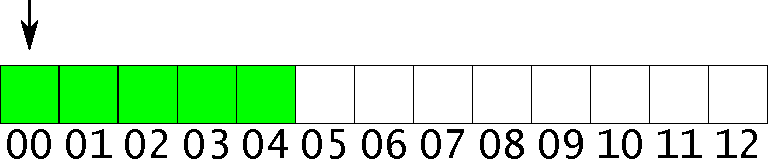
\includegraphics[width=\linewidth]{images/stack_frag_alloc}
	
	\begin{block}{}
		\lstinputlisting[language=C++, linerange=1-1]{cpp-code/objects.cpp}
	\end{block}
	
	Der Stack-Pointer (Pfeil) zeigt auf den nächsten freien Speicherblock.
\end{frame}

\begin{frame}[fragile, t]{Definition von »Dingen«}
	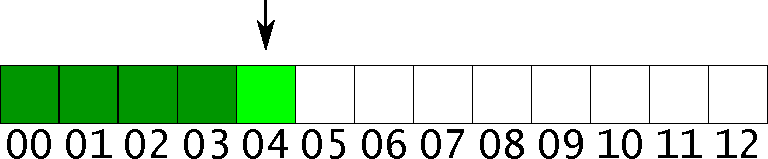
\includegraphics[width=\linewidth]{images/stack_frag_store}
	
	\vspace{1em}
	
	Alle Definitionen legen »Dinge« auf dem Stack an.\\
	{\tiny Ausnahme: \verb|static|}
	
	{\footnotesize
	\begin{block}{}
		\lstinputlisting[language=C++, linerange=3-6]{cpp-code/objects.cpp}
	\end{block}
	}
\end{frame}

\begin{frame}[fragile, t]{Direkter Zugriff auf »Dinge«}
	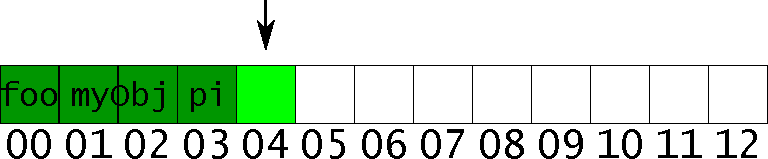
\includegraphics[width=\linewidth]{images/object_names}
	
	\vspace{1em}
	
	Der Compiler kann den Namen des »Dings« direkt verwenden, d.h. in einer Operation auf den Speicher zugreifen.
	
	{\footnotesize
	\begin{block}{}
		\lstinputlisting[language=C++, linerange=8-8]{cpp-code/objects.cpp}
	\end{block}
	}
\end{frame}

\begin{frame}[fragile, t]{Indirekter Zugriff auf »Dinge«}
	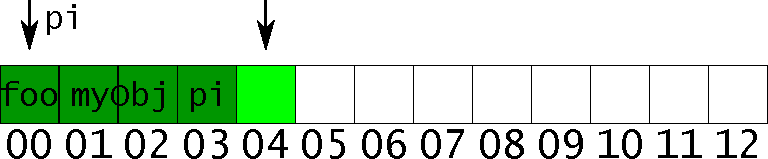
\includegraphics[width=\linewidth]{images/object_points}
	
	\vspace{1em}
	
	Pointer haben zum Inhalt die Adresse eines »Dings«.
	
	{\footnotesize
	\begin{block}{}
		\lstinputlisting[language=C++, linerange=10-10]{cpp-code/objects.cpp}
	\end{block}
	}
\end{frame}

\begin{frame}[fragile, t]{Entfernen von »Dingen«}
	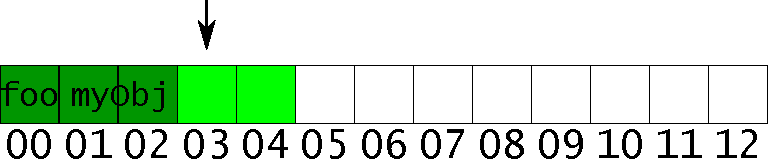
\includegraphics[width=\linewidth]{images/object_pop}
	
	\vspace{1em}
	
	Endet der Block, in welchem ein »Ding« definiert wurde, wird es weggeräumt.
	
	{\footnotesize
	\begin{block}{}
		\lstinputlisting[language=C++, linerange={5-6, 11-12}]{cpp-code/objects.cpp}
	\end{block}
	}
\end{frame}

\begin{frame}{Reihenfolge des Entfernens von »Dingen«}
	Aufgrund der Architektur des Stacks werden die »Dinge« in der Reihenfolge weggeräumt, in dem sie erzeugt wurden.
	
	\pause
	\vspace{1em}
	
	Weitere Besonderheit der Implementierung: Alle Speicherreservierungen im Blocks auf dem Stack können gleichzeitig vorgenommen werden, und zwar zu Beginn des Blocks.
\end{frame}


\subsection{Fragmentierung des Stacks?}

\stackimgframe{Leerer Speicher}{free}{}

\stackimgframe{Alloziere einen Stack}{stack_frag_alloc}{
	\lstinputlisting[language=C++, linerange=1-1]{cpp-code/stack.cpp}
}

\stackimgframe{Belege den Stack (push)}{stack_frag_store}{
	\lstinputlisting[language=C++, linerange=3-6]{cpp-code/stack.cpp}
}

\stackimgframe{Entferne vom Stack (pop)}{stack_frag_pop}{
	\lstinputlisting[language=C++, linerange=3-7]{cpp-code/stack.cpp}
}

\stackimgframe{Voller Stack}{stack_frag_pre_realloc}{}

\stackimgframe{Alloziere mehr Speicher für den Stack}{stack_frag_realloc}{}

\stackimgframe{Belege mehr Stack}{stack_frag_more_store}{}

\stackimgframe{Entferne vom Stack}{stack_frag_dealloc}{}

\stackimgframe{Fragmentierter Stack}{stack_frag_full}{}


\subsection{Heap}

\begin{frame}[fragile]{Allokation auf dem Heap}
	\verb|new TYPE;| \hspace{1em} bzw. \hspace{1em} \verb|new TYPE(PARAMETER);|
	\begin{itemize}
		\item Alloziert das »Ding« auf dem Heap (den Speicher!).
		\item Ruft den Konstruktor von TYPE auf (und übergibt die PARAMETER).
		\item Gibt die Adresse des Speichers zurück, als \verb|TYPE*|.
	\end{itemize}
	
	\vspace{2em}
	
	\verb|new TYPE[DYNAMIC_NUMBER];| -- die Variante mit Parametern \emph{existiert nicht!}
	\begin{itemize}
		\item Alloziert \verb|DYNAMIC_NUMBER| »Dinge« auf dem Heap (den Speicher!).
		\item Ruft für jedes Element den \emph{default}-Konstruktor von TYPE auf.
		\item Gibt die Adresse des Speichers des nullten Elements zurück, als \verb|TYPE*|.
	\end{itemize}
\end{frame}

\begin{frame}[fragile]{Deallokation vom Heap}
	\verb|delete ADDRESS;| -- ADDRESS muss eine Rückgabe von \verb|new| sein, sei hier vom Typ TYPE*
	\begin{itemize}
		\item Ruft den Dekonstruktor vom Objekt auf (\verb|ADDRESS->~TYPE();|)
		\item Dealloziert den Speicher vom Heap.
	\end{itemize}
	
	\vspace{2em}
	
	\verb|delete[] ADDRESS;| -- ADDRESS muss eine Rückgabe von \verb|new [...]| sein
	\begin{itemize}
		\item Ruft den Dekonstruktor jedes Elementes auf.
		\item Dealloziert den Speicher vom Heap.
	\end{itemize}
\end{frame}

\stackimgframe{Leerer Speicher}{free}{}

\stackimgframe{Alloziere einen Stack fester Größe}{stack_heap_alloc}{
	\lstinputlisting[language=C++, linerange=1-1]{cpp-code/stack.cpp}
}

\stackimgframe{Belege den Stack}{stack_heap_store}{
	\lstinputlisting[language=C++, linerange=14-16]{cpp-code/stack.cpp}
}

\stackimgframe{Alloziere auf dem Heap}{stack_heap_alloc_plusheap}{
	\lstinputlisting[language=C++, linerange=18-21]{cpp-code/stack.cpp}
}

\stackimgframe{Fragmentierter Heap}{stack_heap_frag}{
	\lstinputlisting[language=C++, linerange=23-25]{cpp-code/stack.cpp}
}

\stackimgframe{Defragmentierter Heap}{stack_heap_defrag}{
	\lstinputlisting[language=C++, linerange=23-26]{cpp-code/stack.cpp}
}

\begin{frame}[fragile]{Storage duration}
	Der C++ Standard kennt weder Stack noch Heap, dafür aber eine \emph{Speicherdauer der »Dinge«} (storage duration of objects).
	
	\vspace{1em}
	
	\begin{block}{automatic storage duration}
		Das »Ding« wird bei der Definition angelegt und beim Ende des Blocks weggeräumt $\rightarrow$ Stack
	\end{block}
	
	\vspace{1em}
	
	\begin{block}{dynamic storage duration}
		Man muss das »Ding« selbst erzeugen (\verb|new|) und selbst wegräumen (\verb|delete|).
	\end{block}
\end{frame}

\begin{frame}[fragile]{Stack vs. Heap}
	\begin{block}{Stack}
		\begin{itemize}
			\item Schnelle Allokation \& Deallokation {\tiny(z.B. ein einzige Operation für beliebig viel »Dinge«!)}
			\item Direkter, schneller Zugriff
			\item Optimierungen gut und einfach(er) für den Compiler
			\item Erzeugung \& Aufräumen ist automatisch
			\item Begrenzter Speicher (z.B. 1~MB auf Desktop-Rechner)
			\item Größe des »Dings« und Anzahl muss dem Compiler bekannt sein
		\end{itemize}
	\end{block}
	
	\begin{block}{Heap}
		\begin{itemize}
			\item Für große »Dinge«
			\item Eigene Verwaltung der Speicherdauer
			\item Speicherverwaltung während das Programm läuft
		\end{itemize}
	\end{block}
\end{frame}

